\documentclass{beamer}
\usetheme{Boadilla}

\usepackage{algorithm2e}
\usepackage{amsmath}
\usepackage{amsfonts}
\usepackage{hyperref}

\usepackage{amsmath}
\DeclareMathOperator*{\argmax}{arg\,max}
\DeclareMathOperator*{\argmin}{arg\,min}


\title{Probabilistic Circuits:
A Unifying Framework for Tractable Probabilistic Models}
\author{Parviz Karimov}
\institute{MIPT, 2023}


\begin{document}

\begin{frame}
    \titlepage
\end{frame}


\begin{frame}
    \tableofcontents
\end{frame}


\section{Motivation \& Background}

\begin{frame}{Motivation}
    \begin{block}{}
         The increased expressiveness of these probabilistic models, and the ability of
        modern neural density estimators of scaling learning to large amounts of data comes with the inability to perform reliable and efficient probabilistic inference in all
        but the most trivial of probabilistic reasoning scenarios. These
        models resort to various approximation techniques for answering basic questions about the
        probability distributions they represent.
        As the models get closer to fitting the true distribution with high fidelity, we are also getting further away from our goal of solving problems by
        probabilistic reasoning, to some extent nullifying the very purpose of probabilistic modeling
        and learning.
    \end{block} 
\end{frame}


\begin{frame}{Background}
	\begin{block}{Probabilistic model}
        A \textbf{probabilistic model} is a particular representation of a probability distributions. For
        a probabilistic model m that has parameters $\theta$, we will use either $p_m(\mathbf{X})$ or $p_{\theta}(\mathbf{X})$ to denote
        the probability distribution that is represented by the probabilistic model.
	\end{block}
    
    \begin{block}{Query}
        Questions that involve computing some quantities of interest of the joint probability distribution are called \textbf{queries}.
    \end{block}
\end{frame}

\section{Definitions}
\begin{frame}{Definitions}
    \begin{block}{Tractable probabilistic inference}
        A class of queries $\mathbf{Q}$ is tractable
        on a family of probabilistic models $\mathcal{M}$ iff any query $q \in \mathbf{Q}$ on a model $m \in \mathcal{M}$ can be
        computed in time $\mathcal{O}(poly(|m|))$. We also say that $\mathcal{M}$ is a tractable model for $\mathbf{Q}$.
    \end{block}

    \begin{block}{Factorized model}
        Consider the probabilistic model $m$ encoding a joint
        probability distribution over a collection of RVs $X = \bigcup_{i = 1}^{k} \mathbf{X}_i$ partitioned into disjoint sets
        $\mathbf{X}_i \cap \mathbf{X}_j = \emptyset$ for any $i \neq j$ in $1, . . . , k$ where $k > 1$. Model $m$ is a factorized model if
        $$
        p_m(\mathbf{X}) = \prod_{i = 1}^k p_{m_i}(\mathbf{X}_i)
        $$
    \end{block}
\end{frame}
\begin{frame}{Definitions}

    \begin{block}{Mixture model}
        Let $\{p_{m_i}\}_{i = 1}^k$ a finite collection of probabilistic models,
        each defined over the same collection of RVs $\mathbf{X}$. A mixture model is the probabilistic model
        defined as the convex combination
        $$
        p_m(\mathbf{X}) = \sum_{i = 1}^k \theta_i p_{m_i}(\mathbf{X}_i)
        $$
    \end{block}

    \begin{block}{Probabilistic circuits}
        A probabilistic circuit (PC) $\mathcal{C}$ over RVs $\mathbf{X}$,
        is a pair ($\mathcal{G}$, $\mathbf{\theta}$), where $\mathcal{G}$ is a computational graph, also called the circuit structure that
        is parameterized by $\mathbf{\theta}$, also called the circuit parameters, as defined next. The PC $\mathcal{C}$
        computes a function that characterizes a (possibly unnormalized) distrbution $p(\mathbf{X})$.
    \end{block}
    
\end{frame}
\begin{frame}{Definitions}
    \begin{block}{PC structure: scope}
        Let $\mathcal{C}$ = ($\mathcal{G}$, $\mathbf{\theta}$) be a PC over RVs $\mathbf{X}$. The computational graph $\mathcal{G}$ is equipped with a scope function $\phi$ which associates to each unit $n \in \mathcal{G}$ a
        subset of $\mathbf{X}$, i.e., $\phi(n) \subseteq \mathbf{X}$. For each non-input unit $n \in \mathcal{G}$, $\phi(n) = \bigcup_{c \in in(n)}\phi(c)$. The scope
of the root of $\mathcal{C}$ is $\mathbf{X}$.
    \end{block}

    \begin{block}{PC structure: computational units}
        Let $\mathcal{C}$ = ($\mathcal{G}$, $\mathbf{\theta}$) be a PC over RVs
        $\mathbf{X}$. Each unit $n \in \mathcal{G}$ encodes a non-negative function $\mathcal{C}_n$ over its scope: $\mathcal{C}_n : \mathrm{val}(\phi(n)) \rightarrow \mathbb{R}_{+}$.
        An input unit $n \in \mathcal{C}$ encodes a non-negative function that has a support $\mathrm{supp}(\mathcal{C}_n)$ and is
        parameterized by $\mathbf{\theta}_n$.
        A product unit $n$ defines the product $\mathcal{C}_n (\mathbf{X}) = \prod_{c \in in(n)}
        \mathcal{C}_c(\mathbf{X})$. A
        sum unit $n$ defines the weighted sum $\mathcal{C}_n(\mathbf{X}) = \sum_{c \in in(n)}
        \mathbf{\theta}_{n,c}\mathcal{C}_c(\mathbf{X})$ parameterized by weights $\theta_{n, c} \geq 0$.
    \end{block}
\end{frame}

\begin{frame}{Definitions}
    \begin{block}{Recursive definition of PCs}
        A PC $\mathcal{C}$ over RVs $\mathbf{X}$ is one of the following:
        \begin{enumerate}

            \item a tractable distribution over $\mathbf{X}$ encoded as a distribution unit,
            \item a product of PCs over subsets of $\mathbf{X}:
            \mathcal{C}(x) = \prod_i \mathcal{C}_i(x)$, or
            \item a positive weighted sum of PCs over subsets of  $\mathbf{\mathbf{X}}: \mathcal{C}(x) = \sum_i w_i\mathcal{C}_i(x)$, with $w_i > 0$.
        \end{enumerate}
    \end{block}

    \begin{figure}
        \centering
        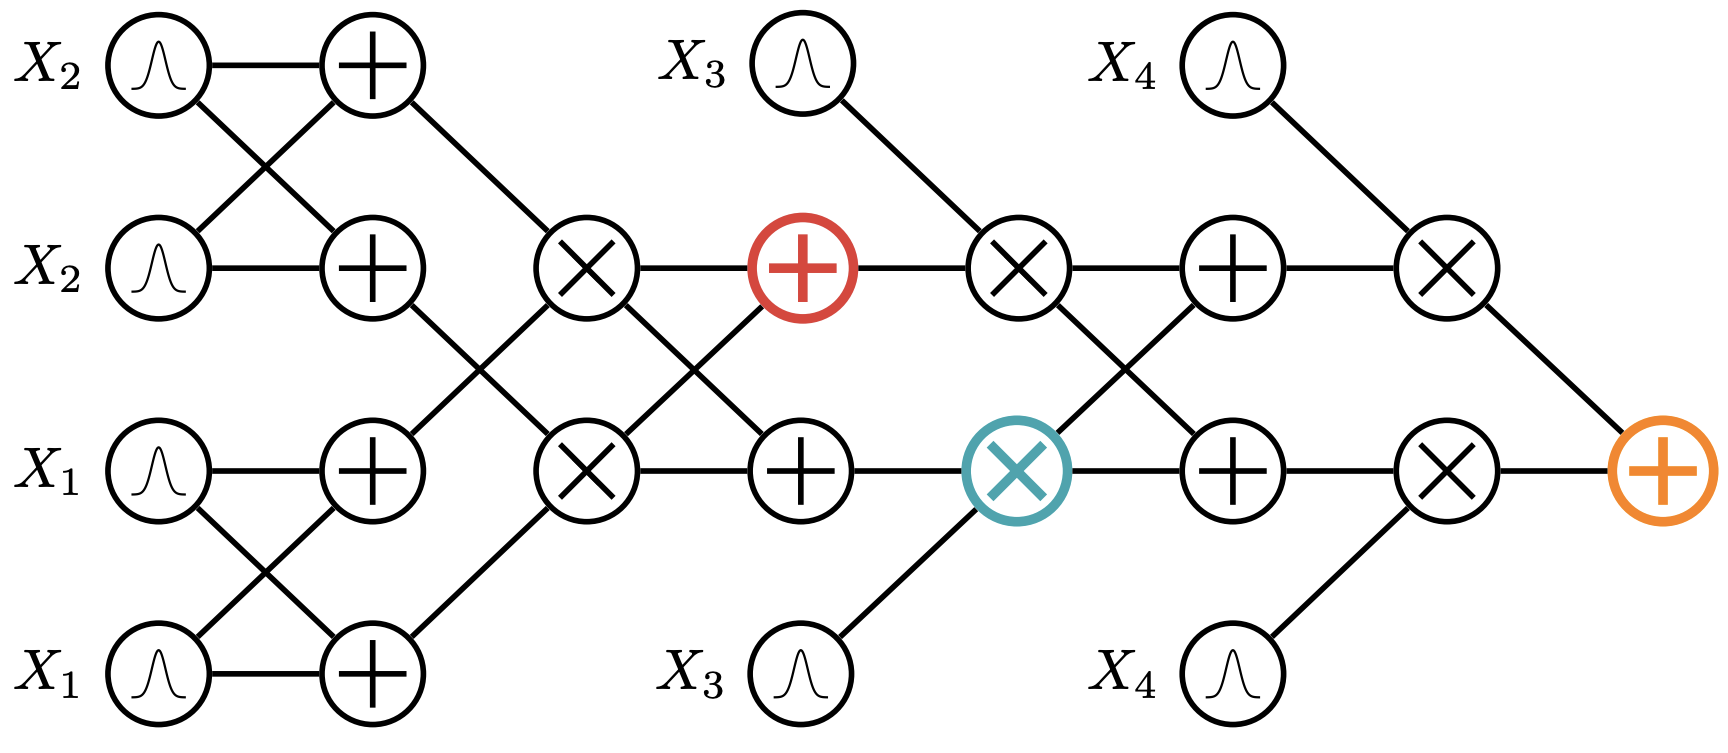
\includegraphics[width=0.5\linewidth]{fst.png}
        \caption{An example of PC}
        \label{fig:pc-example}
    \end{figure}
\end{frame}

\section{Algorithms & results}
\begin{frame}{EVIQuery algorithm}
    \begin{algorithm}[H]
        \caption{EVIQuery(\mathcal{C, x})}

        \KwData{a PC $\mathcal{C} = (\mathcal{G}, \theta)$ over RVs $\mathbf{X}$ and a complete state $x \in \mathrm{val}(\mathbf{X})$}
        \KwResult{$\mathcal{C}(x) := p(\mathbf{X} = x)$}
        $N \gets FeedforwardOrder(\mathcal{G})$\\
        \ForEach {$n \in N$}{
        if $n$ is a sum unit then $r_n \gets \sum_{c \in in(n)}\theta_{n, c}r_c$;\\
        else if $n$ is a product unit then $r_n \gets \prod_{c \in in(n)} r_c$;\\
        else if $n$ is an input distribution then $r_n \gets \mathcal{C}_n(x_{\phi(n)})$\\
        }
        \KwRet $r_n$
    \end{algorithm}
\end{frame}
\begin{frame}{EVIQuery algorithm}
\begin{figure}
    \centering
    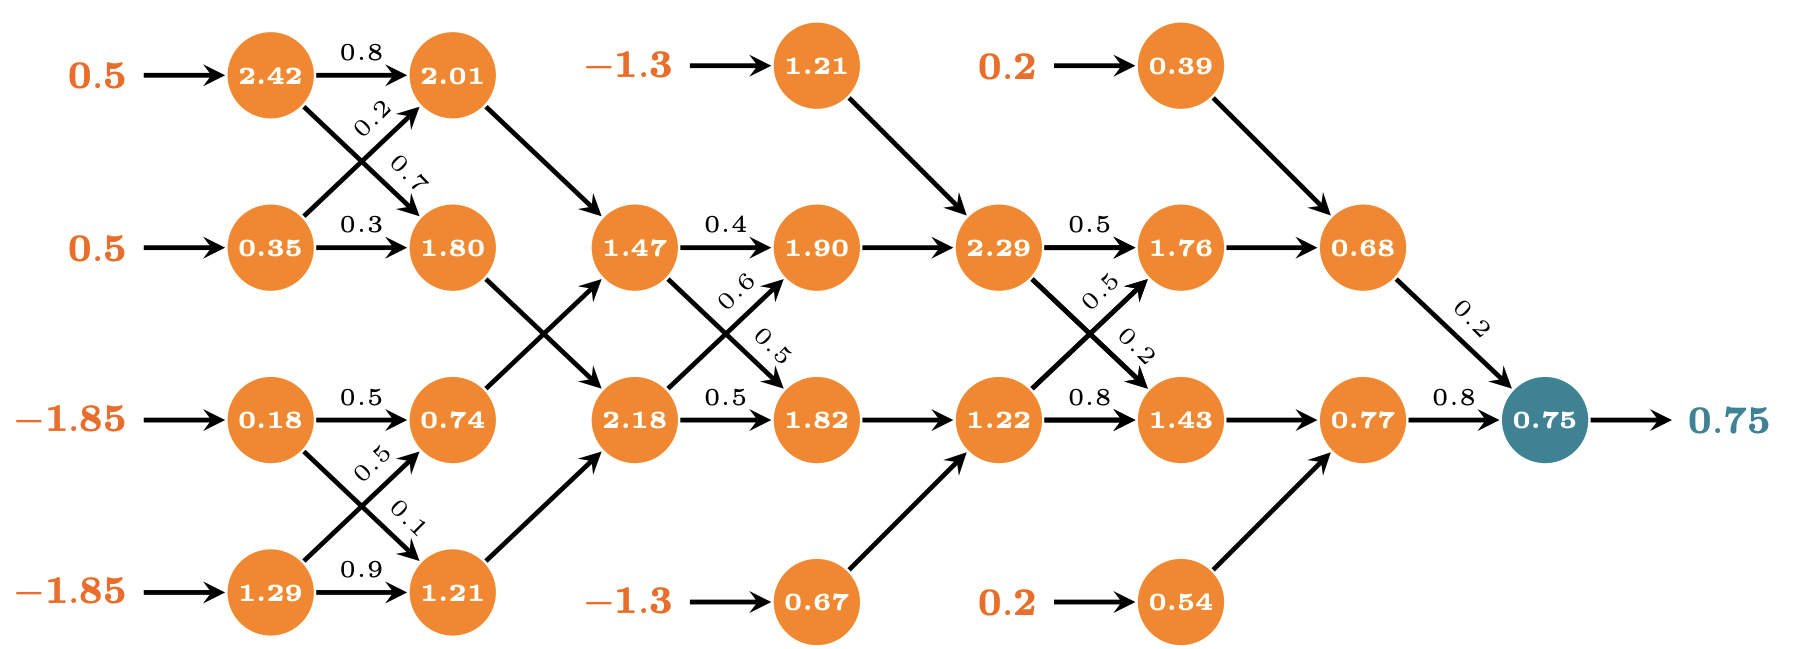
\includegraphics[width=0.7\linewidth]{snd.png}
    \caption{EVIQuery algorithm}
    \label{fig:EVIQuery-algo}
\end{figure}
\end{frame}

\begin{frame}{MAP algorithm}
    \begin{algorithm}[H]
        \caption{MAP(\mathcal{C, e})}

        \KwData{a PC $\mathcal{C} = (\mathcal{G}, \theta)$ over RVs $\mathbf{X}$ and a complete state $e \in \mathrm{val}(\mathbf{E})$} for $\mathbf{E} \subseteq \mathbf{X}$\\
        \KwResult{$\max_{q \in \mathrm{val}(\mathbf{Q})}\mathcal{C}(q, e)$ for $\mathbf{Q} = \mathbf{X} \backslash \mathbf{E}$}
        $N \gets FeedforwardOrder(\mathcal{G})$\\
        \ForEach {$n \in N$}{
        if $n$ is a sum unit then $r_n \gets \max_{c \in in(n)}\theta_{n, c}r_c$;\\
        else if $n$ is a product unit then $r_n \gets \prod_{c \in in(n)} r_c$;\\
        else if $n$ is an input distribution then $r_n \gets \mathcal{C}_n^{max}(e_{\phi(n)})$\\
        }
        \KwRet $r_n$
    \end{algorithm}
\end{frame}

\begin{frame}{PC and other models}
    \begin{block}{PCs are not PGMs}
        Classical PGMs (ex. BNN, MRF) have a clear representational semantics, while
        the semantics of PCs is clearly operational.
        That is, units in the computational graphs of
        PCs directly represent how
        to answer probabilistic queries. On the other hand, nodes in a graph of a PGM denote RVs.
    \end{block}

    \begin{block}{PCs are neural networks}
        Computational graphs in PCs are peculiar NNs where neurons are constrained
        to be either input distribution, sum or product units. As such, a PC is a NN containing two forms of non-linearity: the first provided by the
        input distribution units warping inputs via their densities or masses, the second by the
        product units.
    \end{block}
\end{frame}
\begin{frame}{PC and other models}
    \begin{block}{PCs are hierarchical mixture models}
        a smooth PC as marginalizing out a categorical LV
        associated to each of its sum units. As a result, PCs are hierarchical latent variable models,
        and more precisely deep mixture models. In the following we discuss the LV semantics of
        PCs and what it entails.
    \end{block}
    \begin{figure}
        \centering
        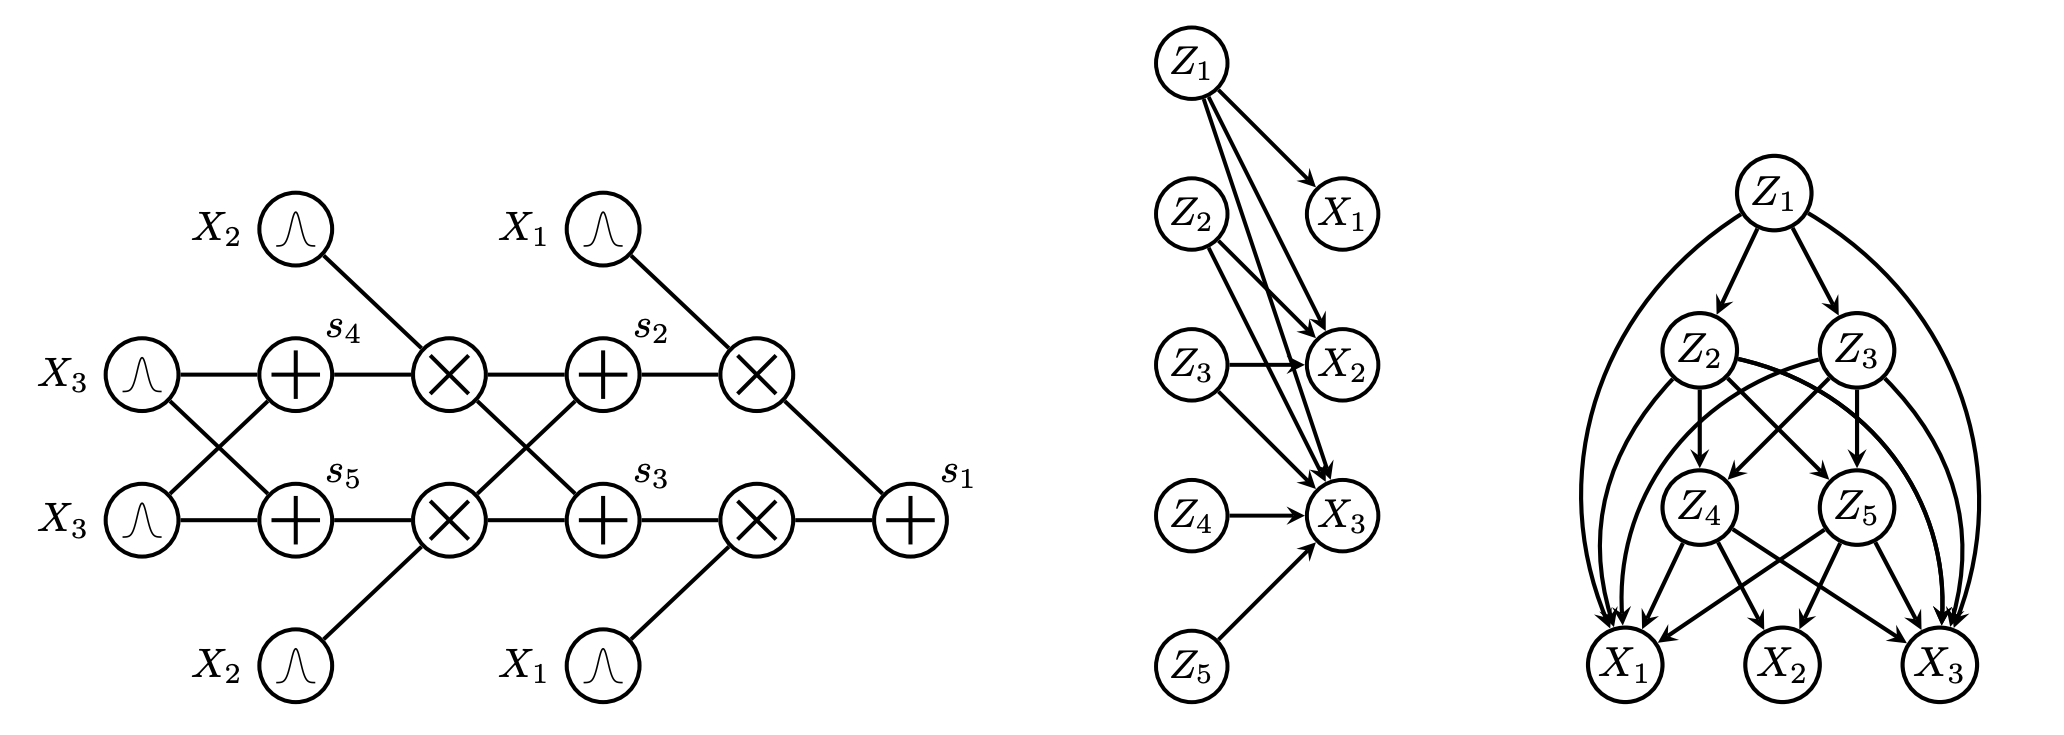
\includegraphics[width=0.8\linewidth]{trd.png}
        \caption{PC as HMM}
        \label{fig:pc-as-hmm}
    \end{figure}
\end{frame}

\begin{frame}{Literature}
    \begin{enumerate}
        \item \textbf{Main article} \href{http://starai.cs.ucla.edu/papers/ProbCirc20.pdf}
        {Probabilistic ciruits}.
    \end{enumerate}
\end{frame}



\end{document}
